{\sl This fieldstone was developed in collaboration with Rens Elbertsen}. \index{Rens Elbertsen}

This is based on the community benchmark for viscoplastic thermal convection
in a 2D square box \cite{tosn15} as already carried out in \ref{f_28}.

In this experiment the geometry is an annulus of inner radius 
$R_1=1.22$ and outer radius $R_2=2.22$. 
The rheology and buoyancy forces are identical to those of the box 
experiment. The initial temperature is now given by:
\[
T(r,\theta) = T_c(r)+A\; s(1-s) \cos(N_0 \theta)
\quad\quad s=\frac{R_2-r}{R_2-R_1} \in [0,1]
\]
where $s$ in the normalised depth, $A$ is the amplitude of the perturbation and $N_0$ the 
number of lobes. In this equation $T_c(r)$ stands for the steady state purely conductive 
temperature solution which is obtained by solving the Laplace's equation in 
polar coordinates (all terms in $\theta$ are dropped because of radial symmetry) 
supplemented with two boundary conditions:
\[
\Delta T_c = \frac{1}{r}\frac{\partial }{\partial r} \left( r \frac{\partial T}{\partial r} \right) =0 
\quad\quad
\quad\quad
T(r=R_1)=T_1=1
\quad\quad
\quad\quad
T(r=R_2)=T_2=0
\]
We obtain 
\[
T_c(r)=\frac{\log (r/R_2)}{\log(R_1/R_2)}
\]
Note that this profile differs from the straight line that is used in \cite{tosn15} and in section \ref{f28}.

\begin{center}
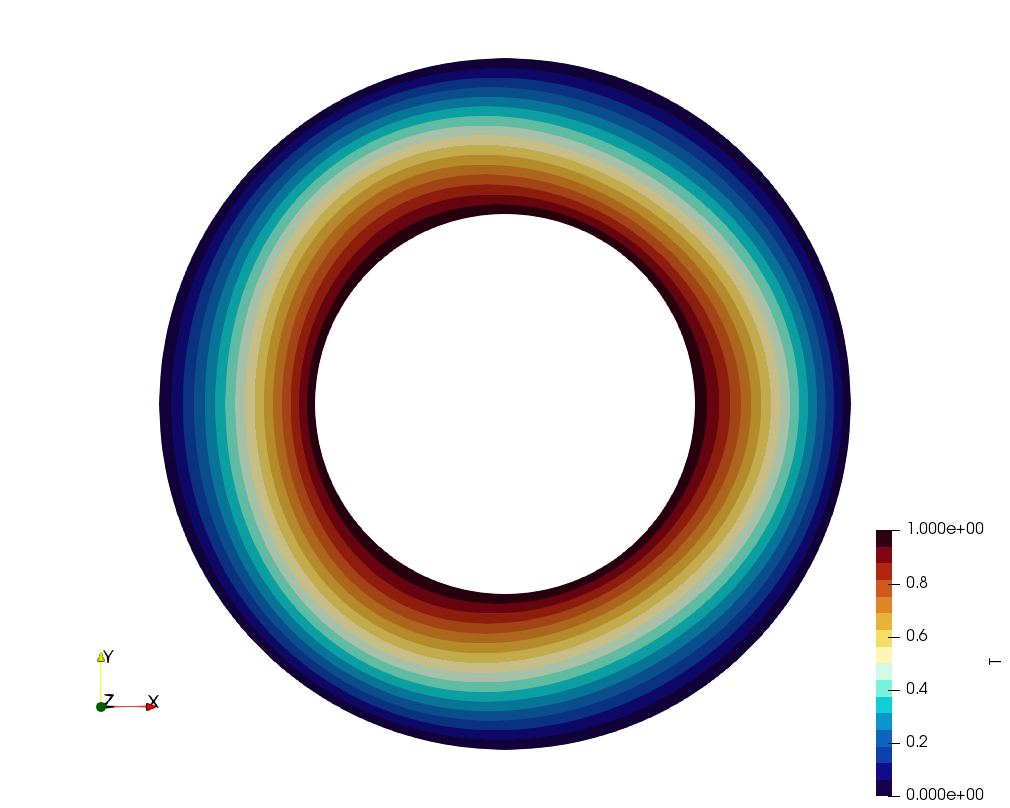
\includegraphics[width=4cm]{python_codes/fieldstone_33/images/T_N03}
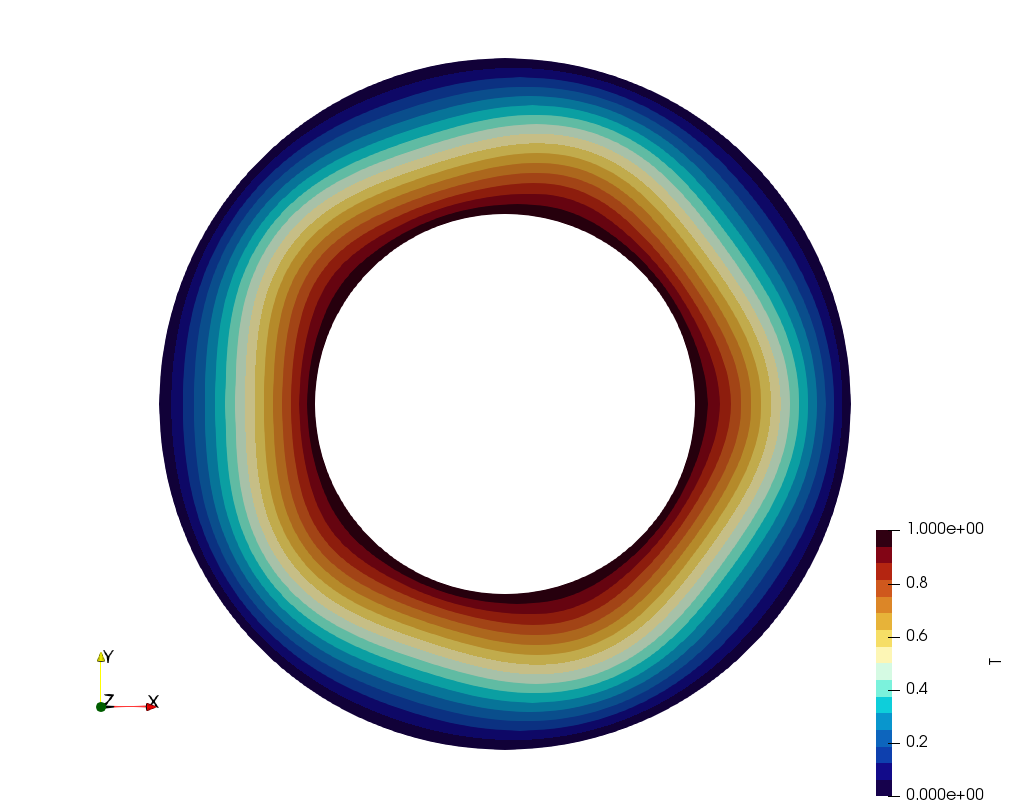
\includegraphics[width=4cm]{python_codes/fieldstone_33/images/T_N05}
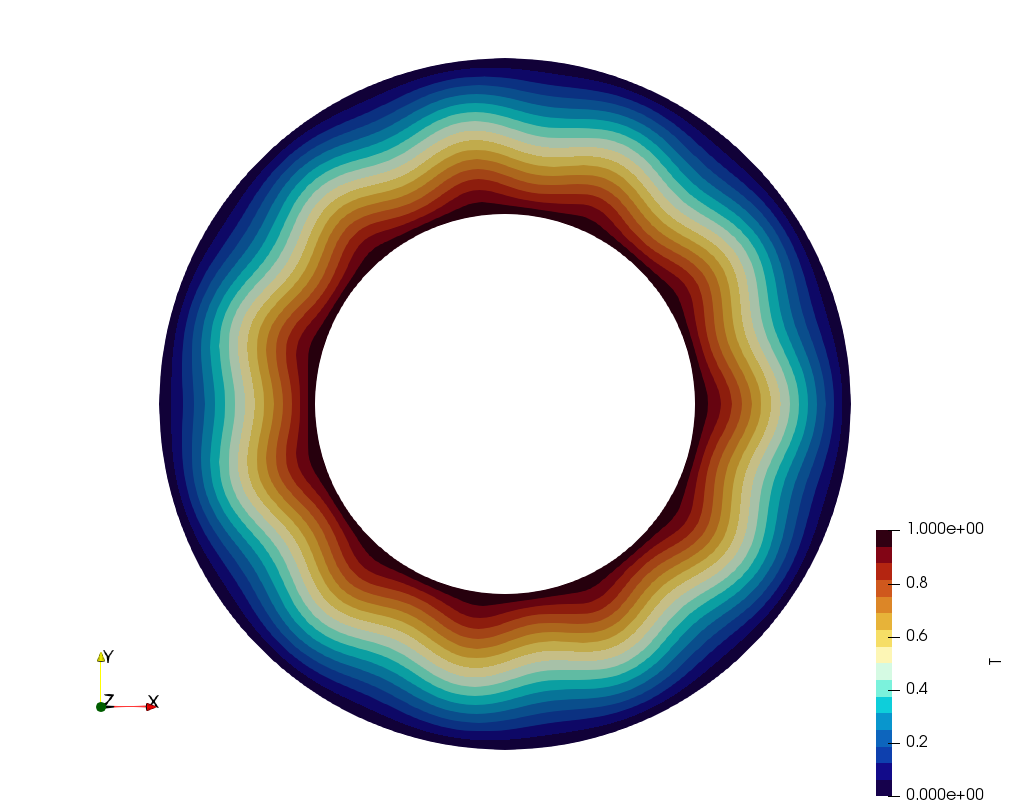
\includegraphics[width=4cm]{python_codes/fieldstone_33/images/T_N11}\\
{\small Examples of initial temperature fields for $N_0=3,5,11$}
\end{center}

Boundary conditions can be either no-slip or free-slip on both inner and outer boundary. However, when free-slip 
is used on both a velocity null space exists and must be filtered out. In other words,
the solver may be able to come up with a solution to the Stokes operator, but 
that solution plus an arbitrary rotation is also an equally valid solution.
This additional velocity field can be problematic since it is used for advecting temperature (and/or compositions)
and it also essentially determines the time step value for a chosen mesh size (CFL condition).

For these reasons the nullspace must be removed from the obtained solution after every timestep.
There are two types of nullspace removal: removing net angular momentum, and removing net rotations.




We calculate the following output parameters: 
\begin{itemize}
\item the average temperature $<T>$
\begin{equation}
\langle T \rangle = \frac{\int_\Omega T  d\Omega }{\int_\Omega d \Omega }
=\frac{1}{V_\Omega}\int_\Omega T d\Omega
\end{equation}
\item the root mean square velocity $v_{rms}$ as given by equation (\ref{eqVrms}).
\item the root mean square of the radial and tangential velocity components as given by equations (\ref{eqVrVrms}) and (\ref{eqThetaVrms}).
\item the heat transfer through both boundaries $Q$:
\begin{equation}
Q_{inner, outer} = \int_{\Gamma_{i,o}} \boldsymbol{q} \cdot \boldsymbol{{n}} \; d\Gamma 
\end{equation}
\item the Nusselt number at both boundaries $Nu$ as given by equations (\ref{eqNuAnnIn}) and  (\ref{eqNuAnnOut}). 
\item the power spectrum of the temperature field:
\begin{equation}
PS_n(T) = \left |\int_\Omega T(r, \theta) e^{in\theta} d\Omega \right |^2.
\end{equation}
\end{itemize}




\fbox{
\parbox{10cm}{{\bf features}
\begin{itemize}
\item $Q_1\times P_0$ element
\item incompressible flow
\item penalty formulation
\item Dirichlet boundary conditions
\item non-isothermal
\item non-isoviscous
\item annulus geometry
\end{itemize}
}}




